\section{Introduction}
\label{sec::introduction}

The deafening and thunderous sound of the current eSports scene is getting more and more common each year that goes by and so is its volume as the latest The International event for Dota shows in the tremendous prize pool of almost 25 million dollars \citep{esportsEarnings}.\\


\begin{figure}
\begin{center}
\fbox{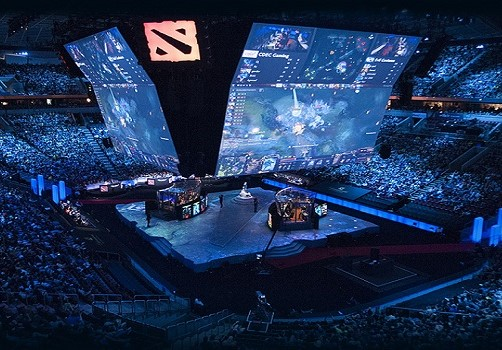
\includegraphics[width=0.95\linewidth]{resources/theInternational_2.jpg}}

	\caption{The International 2017. Image from \href{http://www.gosugamers.net/dota2/news/44947-the-international-2017-prize-pool-shatters-ti6-record}{\nolinkurl{gosugamers.net}}}
\end{center}
\end{figure}



We got used to colossal games and titanic multimillion events happening every year involving eSports competitions. But every story has its beginning and this one is no different.\\

Back in the 90s when eSports, as they are today, could only be imagined or dreamed of one game and its players started to lay the first few stones. \textbf{Quake} and its small but enthusiastic fan-base had a very significant impact in creating the foundation of the competitive gaming scene and, as such, they gained the right to be considered amongst the \textit{Grandfathers of eSports}.\\

\subsection{Defining eSport}

Before jumping into the core of the content regarding Quake it is necessary to have a common idea of what the term \textbf{eSports} means in the current context. Commonly defined as any form of competition facilitated by video-games, that definition would be slightly distant from the real meaning that it tends to have between players. When someone that knows about the eSports scene thinks about examples of what an eSport actually is games such as \textbf{\textit{League of Legends}} \citep{game:league}, \textit{\textbf{Counter-Strike}} \citep{game:cs}, \textbf{\textit{Starcraft}} \citep{game:starcraft} or \textit{\textbf{Street Fighter}} \citep{game:streetfighter} generally come to mind.\\

The common factor that these games have that the definition ignores is the fact that they all involve \textbf{direct competition} against other players. This distinction is important in the context of the present topic since it leaves out of the eSports definition the competitive arcade game scene in the 80s.\\

Games such as \textbf{\textit{Pac-Man}} \citep{game:pacman} or \textbf{\textit{Donkey Kong}} \citep{game:donkeykong} had significant competition before the 90s as documented in The King of Kong \citep{kingKong}. But this type of \textbf{indirect competition} in which players try to perform better than their opponent against the machine is not very correlated to the current common eSports definition. A good argument for this is the fact that the top 100 games by prize money \citep{biggestEsports} (softly correlated to player counts and view numbers) does not list a single game that involves \textbf{indirect competition}, all of them have a direct players versus player model.\\

Having this in mind, a good short and simple although not necessarily universal definition would be:\\

\begin{center}
\textbf{\textit{Direct video-game competitions often played for on-line or live audiences}}
\end{center}

\subsection{Introducing Quake}

Terms such as \textit{Arcade Style Shooter}, \textit{Arena-FPS} or \textit{Ego-Shooter} are commonly used to describe what Quake is. Understanding what this means is important to then be able to fully grasp why the story started and ended the way it did.\\

This game was about highly enthusiastic communities, almost reaching a somewhat healthy version of fanaticism. It came to tap into the deeply rooted but unsatisfied desire for real competition that these players had. Previously there were things such as the already mentioned arcade game tournaments but those lacked the thrill of directly defeating your opponent with your superior skills \parencite[p.~7]{taylor2012raising}. And games such as \textit{Doom} \citep{game:doom} that offered similar game-play were significantly worse regarding the technology, availability, level of competition and more factors expanded in the next sections.\\

Here it is where the very interesting definition of \textbf{\textit{Ego-Shooter}} comes into play. Surprisingly enough, that is the translation of First-person shooter for the German language. The word \textit{Ego} here started without the usual meaning related to valuing oneself too highly but slowly morphed towards there when English speaking European players found out how well this fitted the game and its players.\\

The design of this game made it so mastery was difficult but satisfactory. This high skill ceiling is one of \textit{Quake}'s most notorious characteristics even today and it made competing against similarly passionate opponents especially attractive. Even more so than the few previous directly competitive games that came before such as the first \textit{\textbf{Street Fighter}} \citep{game:streetfighter2}.\\

\subsubsection{Why not others?}

Given that our definition already excludes indirectly competitive arcade games the only truly relevant contender for the title of \textit{Grandfather of eSports} is the game that was just mentioned: \textbf{\textit{Street Fighter II}} \citep{game:streetfighter2}.\\

Two games from the \textit{Street fighter} franchise were the ones involved in the first \textit{Evolution Championship Series} in 1996. There are two main reasons why Quake's run in the late 90s makes it more relevant than \textit{Street Fighter}.\\

The first one is the raw size, visibility and quality of the first real Street Fighter tournament, \textbf{B3}\footnote{\textbf{B3: Battle by the Bay}\citep{evo} was the first tournament organized by the now known as \textbf{Evolution Championship Series}}. There were roughly 40 players involved and the matches were not shown on-line or to a significant live audience besides the players themselves. The only way to see some of the matches was with VHS recordings.\\

The other significant reason is that there was not another significant competition for \textit{Street fighter} until the year 2000 where another \textit{\textbf{Battle by the Bay}} tournament, the \textbf{B4}, was organized. This shows the \textbf{lack of impact} that this game had when compared to the big events that Quake had starting in 1997 with thousands of people in a live audience, high production value on-line streaming and big prize money.
